\documentclass[supercite]{Experimental_Report}
\title{~~~~~~信息技術導論~~~~~~}
\author{阮云轩}
%\coauthor{张三、李四}
\school{计算机科学与技术学院}
\classnum{CS2404}
\stunum{U202490035}
%\costunum{U202115631、U202115631}
\instructor{余辰} % 该系列实验报告模板由华科大计院教师陈加忠制作
\date{2024年12月18日}

\usepackage{algorithm, multirow}
\usepackage{algpseudocode}
\usepackage{amsmath}
\usepackage{amsthm}
\usepackage{framed}
\usepackage{mathtools}
\usepackage{subcaption}
\usepackage{xltxtra} %提供了针对XeTeX的改进并且加入了XeTeX的LOGO, 自动调用xunicode宏包(提供Unicode字符宏)
\usepackage{bm}
\usepackage{tikz}
\usepackage{tikzscale}
\usepackage{pgfplots}
\usepackage{listings}
\usepackage{tocloft}
%\usepackage{enumerate}
\lstdefinestyle{commonCodeStyle}{
	language = C, % 假设主要是C语言代码，可按需更改语言类型
	basicstyle=\ttfamily\footnotesize, % 设置字体为等宽且小一号字体，方便排版
	breaklines = true, % 自动换行
	breakatwhitespace = true, % 尽量在空白处换行
	columns=flexible, % 灵活调整列宽，让代码适应页面宽度
	numbers=left, % 在代码左侧显示行号
	numberstyle=\tiny\color{gray}, % 行号的样式，设置为小字号灰色字体
	keywordstyle=\color{blue}\bfseries, % 关键字样式，加粗蓝色显示
	commentstyle=\itshape, % 注释样式，斜体绿色显示
	stringstyle=\color{magenta}, % 字符串样式，紫红色显示
	showstringspaces=false % 取消显示字符串中的空格，放在正确位置
}

\lstdefinestyle{mycode}{
	language = C,
	basicstyle=\ttfamily,
	breaklines = true,
	breakatwhitespace = true,
	stringstyle=\ttfamily, % 设置字符串的字体风格保持和基本字体一致（等宽字体），这里也可以根据喜好设置其他样式，若不想设置额外样式可不写此行
	showstringspaces=false % 关键在于这一行，用于取消显示字符串中的空格
}
%\usepackage{enumerate}

\pgfplotsset{compat=1.16}

\newcommand{\cfig}[3]{
	\begin{figure}[htb]
		\centering
		\includegraphics[width=#2\textwidth]{images/#1.tikz}
		\caption{#3}
		\label{fig:#1}
	\end{figure}
}

\newcommand{\sfig}[3]{
	\begin{subfigure}[b]{#2\textwidth}
		\includegraphics[width=\textwidth]{images/#1.tikz}
		\caption{#3}
		\label{fig:#1}
	\end{subfigure}
}

\newcommand{\xfig}[3]{
	\begin{figure}[htb]
		\centering
		#3
		\caption{#2}
		\label{fig:#1}
	\end{figure}
}
\renewcommand{\cftlstlistingpresnum}{代码 }
\renewcommand{\cftlstlistingaftersnum}{:}
\setlength{\cftlstlistingnumwidth}{3.5em}

\newcommand{\rfig}[1]{\autoref{fig:#1}}
\newcommand{\ralg}[1]{\autoref{alg:#1}}
\newcommand{\rthm}[1]{\autoref{thm:#1}}
\newcommand{\rlem}[1]{\autoref{lem:#1}}
\newcommand{\reqn}[1]{\autoref{eqn:#1}}
\newcommand{\rtbl}[1]{\autoref{tbl:#1}}

\algnewcommand\Null{\textsc{null }}
\algnewcommand\algorithmicinput{\textbf{Input:}}
\algnewcommand\Input{\item[\algorithmicinput]}
\algnewcommand\algorithmicoutput{\textbf{Output:}}
\algnewcommand\Output{\item[\algorithmicoutput]}
\algnewcommand\algorithmicbreak{\textbf{break}}
\algnewcommand\Break{\algorithmicbreak}
\algnewcommand\algorithmiccontinue{\textbf{continue}}
\algnewcommand\Continue{\algorithmiccontinue}
\algnewcommand{\LeftCom}[1]{\State $\triangleright$ #1}

\newtheorem{thm}{定理}[section]
\newtheorem{lem}{引理}[section]

\makeatletter
% 定义 \subsubsubsection 命令
\newcommand{\subsubsubsection}{\@startsection{subsubsubsection}{4}{\z@}{-3.25ex plus -1ex minus -.2ex}{1.5ex plus.2ex}{\normalfont\Large\bfseries}}
% 定义 \subsubsubsubsection 命令
\newcommand{\subsubsubsubsection}{\@startsection{subsubsubsubsection}{5}{\z@}{-3.25ex plus -1ex minus -.2ex}{1.5ex plus.2ex}{\normalfont\large\bfseries}}
% 定义 \subsubsubsubsubsection 命令
\newcommand{\subsubsubsubsubsection}{\@startsection{subsubsubsubsubsection}{6}{\z@}{-3.25ex plus -1ex minus -.2ex}{1.5ex plus.2ex}{\normalfont\normalsize\bfseries}}
\makeatother

\colorlet{shadecolor}{black!15}

\theoremstyle{definition}
\newtheorem{alg}{算法}[section]

\def\thmautorefname~#1\null{定理~#1~\null}
\def\lemautorefname~#1\null{引理~#1~\null}
\def\algautorefname~#1\null{算法~#1~\null}

\begin{document}
	
	\maketitle
	
	\clearpage
	
	\pagenumbering{Roman}
	
	\tableofcontents[level=2]
	
	\clearpage
	
	\pagenumbering{arabic}
	
	\listoflistings
	\section{摘要}
	
	\subsection{關於行文}
	由于笔者习惯以汉字 (繁体中文) 以行文，在杜撰时经己尽量转换成汉字 (简体中文)，但难免会有汉字 (繁体中文) 的出现。还请读者见谅。\\
	本報告以LateX輯錄而成，部分地方可能出現些許的排版不格範，還請見諒。
	\subsection{前言}
	在当今科技飞速发展的时代，计算机(\ref{pic1-1-1})与人工智能领域正经历着前所未有的变革与突破。在听了这些关于计算器不同领域的相关课程时，使我对这些领域有着诸多深刻的感悟与体会。本报告旨在对计算机和人工智能发展史、大规模存储系统、类脑计算机、计算器通信、通用人工智能技术进展与典型应用以及工程伦理等多方面课程内容进行综合梳理与深度思考。通过对这些主题的回顾与剖析，望能够使读者有深刻的体会理解，更希望自已能够挖掘出它们之间相互交织、相互促进的内在联系，以及理解在推动社会进步的同时所引发的一系列技术、而本报告同时会指出一些计算器相关技术当前面对的问题和难关，如伦理与应用层面的挑战与思考，为进一步深入研究和创新发展提供有益的参考与借鉴。 
	\\由于作者水平有限，难免有些缺点和错误，望广大读者给予批评指正。
	\begin{figure}[H]
		\begin{center}
			
\includegraphics[scale=0.30]{images/1-1.png}
			\caption{IT中國}
			\label{pic1-1-1}
		\end{center}
	\end{figure}

%\begin{lstlisting}[style=commonCodeStyle, caption={示例}, label={lst:0-0}]
%	#include <stdio.h>
%	int main() {
%	printf("Hello, C!\n"); //print out Hello, C!
%	return 0;
%	}
%\end{lstlisting}
%以上是本實驗報告時頻繁出現的編程文本格式，示味着相關的說明部分(\ref{lst:0-0})
	
	\section{计算机和人工智能发展史}
		\subsection{计算机发展}
		下面将会对计算器的发展历程作简单说明，内容包括但不限于计算器发展史，相关突破点，重要时刻，现况和当下挑战等。
		\subsubsection{1930-1950—雄起！}
		计算机可以说是从1930到1950年代开始蓬勃发展的，而Z3 计算机(\ref{pic2-1-1})（1941年）是世界首台可编程电子计算机，实现从机械到电子计算转变，但当时面临电子组件不稳定不可靠问题，通过精心设计电路、采用高质量电子管及严格测试调试解决。1946 年的 ENIAC 作为第一台通用电子计算机用于军事弹道计算，同时因大量电子管发热易故障，靠安装大型空调控温、安排人员维护更换解决。
		\begin{figure}[H]
			\begin{center}
				
\includegraphics[scale=0.30]{images/2-1-1.png}
				\caption{Z3计算机}
				\label{pic2-1-1}
			\end{center}
		\end{figure}
		\subsubsection{1950-1970—集成电路时代}
		紧接着的是1950到1970的晶体管和集成电路时代，在1947年晶体管(\ref{pic2-1-2})的发明可以说是里程碑的重要组成，虽初期生产工艺复杂成本高，但随半导体制造技术发展，改进晶体生长、掺杂、封装等工艺得以改善。1958 年集成电路发明，将多组件集成于芯片大幅缩小计算机体积，依靠高精度光刻技术解决芯片电路连接与组件布局难题。
		\begin{figure}[H]
			\begin{center}
				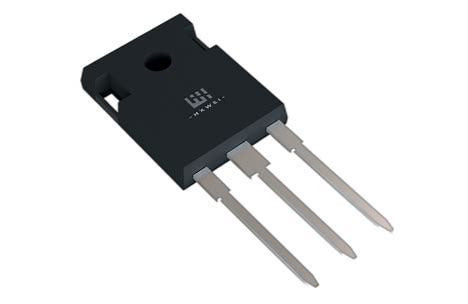
\includegraphics[scale=0.60]{images/2-1-2.jpg}
				\caption{晶体管}
				\label{pic2-1-2}
			\end{center}
		\end{figure}
		\subsubsection{1970-1990—微处理器时代}
		之后的1970到1990年是个人计算机和微处理器时代，1975年Altair 8800(\ref{pic2-1-3}) 引发个人计算机革命，为降低成本采用大规模生产技术、简化设计、选用便宜元器件。1971 年英特尔 4004微处理器将中央处理器集成于芯片，通过优化芯片设计架构与先进半导体制造工艺提升性能。
		\begin{figure}[H]
			\begin{center}
				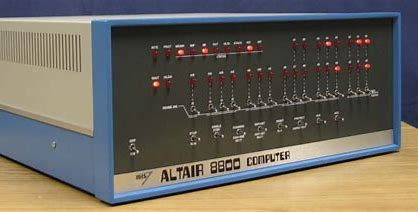
\includegraphics[scale=0.60]{images/2-1-3.jpg}
				\caption{Altair 8800}
				\label{pic2-1-3}
			\end{center}
		\end{figure}
		\subsubsection{1990-至今—现代计算机时代}
		而由1990到现今则是现代计算机时代(\ref{pic2-1-4})，互联网在 1990 年代普及，使计算机可联网共享信息，改变生活工作方式，针对网络安全研发加密、防火墙等技术，为提升数据传输速度升级网络基础设施。2000 年代起移动计算兴起，智能手机和平板出现，通过研发高效电池技术和低功耗芯片设计延长移动设备续航时间，同时优化软件算法和硬件架构提升性能。
		\begin{figure}[H]
			\begin{center}
				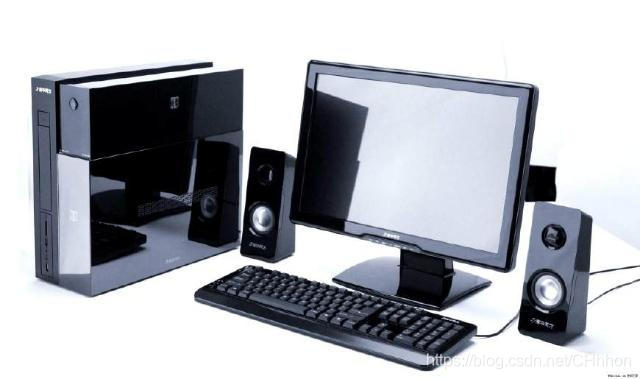
\includegraphics[scale=0.40]{images/2-1-4.jpg}
				\caption{现代计算机时代}
				\label{pic2-1-4}
			\end{center}
		\end{figure}
		\subsubsection{另外小談}
		Web(\ref{pic2-1-5})的誕生—世界的橋樑\\
		特别地说一下，由Web1.0到Web2.0的建成仅用时15年，现在是由Web2.0到Web3.0的发展阶段。互联网技术是一项绝对伟大的技术，是这项技术把世界联系起来的，当时的web1.0还是输入网址才能访问特定的网页资源，用户更多是被动的信息接收者。而 Web2.0 极大改变了这一局面，社交媒体平台蓬勃兴起，用户不仅能便捷地创建和分享自己的内容，如文字、图片、视频等，而且能通过点赞、评论、转发等方式深度参与社交互动，形成了活跃且庞大的虚拟社交网络。在 Web2.0 时代，移动互联网的迅猛发展更是起到了推波助澜的作用，智能手机的普及使得人们可以在任何时间、任何地点接入互联网，各种应用程序如雨后春笋般涌现，涵盖了生活的方方面面，从在线购物、移动支付到在线教育、移动办公等。
		然而，Web2.0 也暴露出诸多问题，比如用户数据的隐私泄露风险日益增加，大型互联网平台垄断了大量的数据资源和用户流量，中小创业者在平台上往往面临高成本、高门坎等困境。而 Web3.0 的出现，正是为了解决这些难题。它基于区块链技术，旨在重新构建互联网的信任机制，使用户真正成为数据的主人，能自主掌控自己的数据使用权和所有权。例如，在去中心化的社交平台中，用户的社交关系和发布的内容不再完全由中心化平台掌控，而是通过区块链的加密和分布式存储技术，保证其安全性和私密性。
		\begin{figure}[H]
			\begin{center}
				
\includegraphics[scale=0.40]{images/2-1-5.jpg}
				\caption{web}
				\label{pic2-1-5}
			\end{center}
		\end{figure}
	
	\subsubsection{前景}
	未来计算机技术会朝着高性能、智能化、绿色化迈进。硬件方面，神经形态计算与量子计算等新型架构若突破，将使计算能力呈指数级跃升，开启新计算时代，像量子计算机在密码破解和复杂科学计算领域会大显身手。软件上，人工智能融入软件开发，达成自动化编程等功能提升开发质效，区块链也会在软件版权、数据安全等多有应用。计算机网络走向高速、低延迟且高可靠，6G 及更先进技术将助力物联网、虚拟现实等大规模普及，促使智能家居、智能交通、智能医疗等领域变革，让生活更便捷、舒适与高效。
	\subsubsection{當下挑戰}
	尽管计算机技术已经取得了巨大成就，但仍面临一些挑战。在硬件层面，随着芯片制程逐渐逼近物理极限，进一步提升芯片性能变得愈发困难，芯片功耗、散热等问题也日益突出。量子计算虽然被视为未来的突破方向，但目前仍处于研发初期，技术成熟度和应用范围有限。在软件方面，软件系统的复杂性不断增加，导致开发周期长、成本高且容易出现漏洞和安全隐患。不同软件和系统之间的兼容性问题也时有发生，给用户带来不便。网络安全更是成为重中之重，计算机网络面临着黑客攻击、数据泄露、恶意软件传播等多种威胁，保障网络安全的技术和措施需要不断更新和完善。此外，随着人工智能等新兴技术对计算资源需求的急剧增加，如何构建更加高效、灵活、绿色的计算基础设施也是待解决的问题。
	
	\subsection{人工智能发展}
	另一个重要的发展史则是人工智能(\ref{pic2-2-1})，以往一般认为人工智能是基于计算器的一门分支学科，但随着其核心的显现，已成为有着与计算器技术相同地位的主流学科
	\begin{figure}[H]
		\begin{center}
			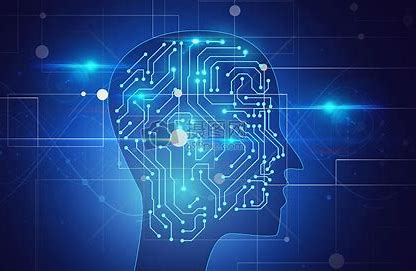
\includegraphics[scale=0.40]{images/2-2-1.jpg}
			\caption{人工智能}
			\label{pic2-2-1}
		\end{center}
	\end{figure}
	\subsubsection{1950-1970}
	自1950至1970年代，人工智能开始起步。1950年图灵测试(\ref{pic2-2-2})的提出，为后续研究确立了目标与评判依据。早期主要围绕符号逻辑与基于规则的系统开展工作，通过编写大量规则去模拟人类思维语言，期望能设计出通过图灵测试的机器。到了1956年达特茅斯会议，标志着人工智能成为独立学科。此后，让计算机具备学习能力成为早期关键任务，由此开启了对机器学习方法在模式识别与分类方面的探索。
	\begin{figure}[H]
		\begin{center}
			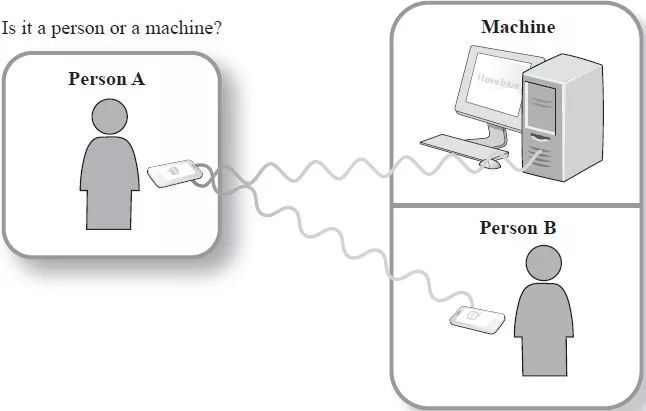
\includegraphics[scale=0.40]{images/2-2-2.jpg}
			\caption{Turning Test}
			\label{pic2-2-2}
		\end{center}
	\end{figure}
	\subsubsection{1970-1980}
	随后进入1970至1980年代，即第一次人工智能寒冬(\ref{pic2-2-3})。当时基于规则的系统在自然语言处理和图像识别等领域遭遇困境。由于计算机计算能力有限，许多算法难以有效施行。在此情况下，研究人员开始反思以往研究方法，并尝试探索神经网络。只是在初期，因缺乏有效训练算法和足够计算资源，神经网络的发展受到较大限制。
	\begin{figure}[H]
		\begin{center}
			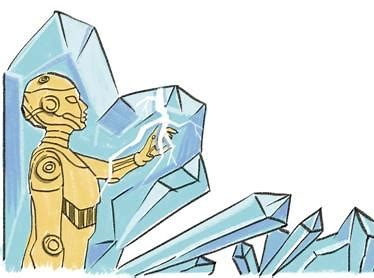
\includegraphics[scale=0.30]{images/2-2-3.jpg}
			\caption{Freeze}
			\label{pic2-2-3}
		\end{center}
	\end{figure}
	\subsubsection{1980-1990}
	接着是1980至1990年代的人工智能复兴时期。1980年代专家系统兴起，它将专家知识经验编码成规则，在多领域取得应用成果。不过，专家系统面临知识获取与表示的难题，为此研究人员通过与专家深入交流合作，并开发多种知识表示方法予以解决。1980 年代后期，神经网络迎来复兴契机，反向传播算法使训练多层神经网络(\ref{pic2-2-4})成为可能。起初，因训练数据不足和计算资源欠缺而面临阻碍，但随着互联网发展，数据获取变得容易，且 GPU 的出现提供了强大计算力，使神经网络得以在语音识别、手写数字识别等领域有所突破。
	\begin{figure}[H]
		\begin{center}
			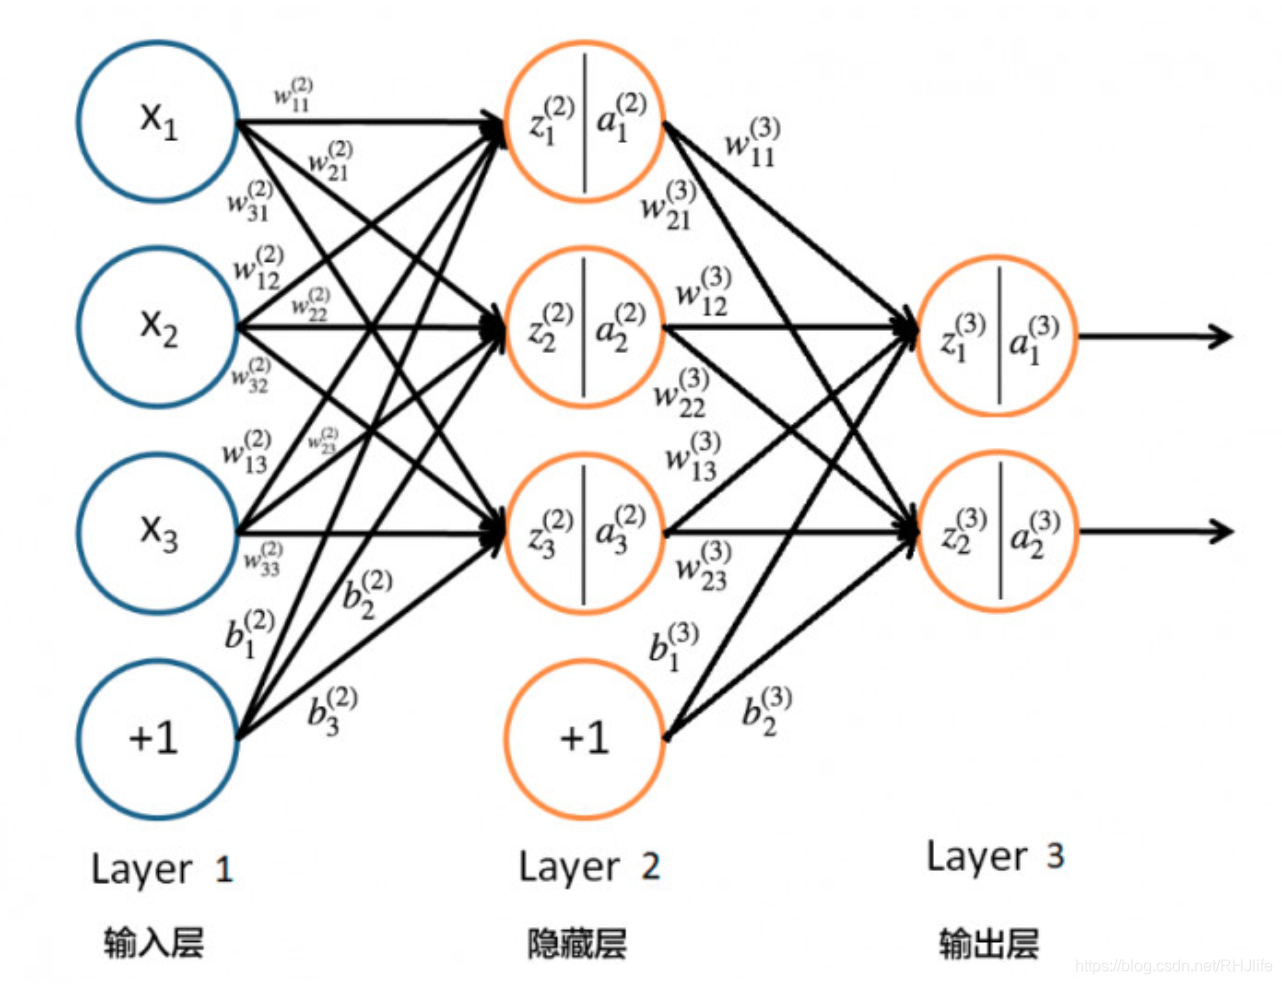
\includegraphics[scale=0.20]{images/2-2-4.png}
				\caption{神经网络}
			\label{pic2-2-4}
		\end{center}
	\end{figure}
	\subsubsection{2010-至今}
	自 2010 年代至今的大数据时代与深度学习(\ref{pic2-2-5})阶段。随着互联网等的发展，大数据兴起，为人工智能训练提供了大量素材。针对数据存储、管理和分析的难题，研发出分布式文件系统和非关系型数据库等用于存储管理，开发各类数据挖掘和机器学习算法来进行分析。深度学习在这一时期崛起，在图像、语音、自然语言处理等领域成果显着。为解决深度学习所需的大量计算资源和标注数据问题，采用了 GPU、TPU 等硬件加速技术与开发分布式训练框架，同时开发数据标注工具以及半监督、无监督学习算法来减少对标注数据的依赖。
	\begin{figure}[H]
		\begin{center}
			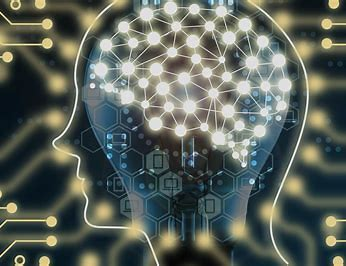
\includegraphics[scale=0.40]{images/2-2-5.jpg}
			\caption{Deep learning}
			\label{pic2-2-5}
		\end{center}
	\end{figure}

	\subsubsection{當下挑戰}
	人工智能的发展也并非一帆风顺。首先是数据依赖问题，深度学习模型需要大量的标注数据进行训练，数据的获取、标注成本高昂且质量难以保证，数据隐私和安全问题也日益凸显。其次，可解释性成为制约人工智能进一步发展的关键因素，深度学习模型如同黑箱，难以理解其决策过程和依据，这在医疗、金融等对决策可靠性要求极高的领域是一个严重的问题。例如，在医疗诊断中，如果人工智能系统做出了错误的诊断，但无法解释原因，医生和患者难以信任和接受。再者，人工智能的伦理和法律问题逐渐暴露，如算法歧视可能导致对某些群体的不公平对待，在就业、信贷等领域可能引发社会矛盾；自动驾驶汽车面临的事故责任界定等伦理困境；以及人工智能创作物的版权归属问题等，都需要建立完善的伦理规范和法律框架来加以约束。此外，人工智能的通用智能水平仍然有限，目前的人工智能系统大多是针对特定任务进行训练和优化，缺乏像人类一样的通用认知和学习能力，难以在复杂多变的环境中灵活应对和自主学习。
	\subsubsection{前景}
	虽面临挑战，人工智能前景仍广阔。技术研发上，探索可解释性方法，开发可视化工具与可解释模型架构，无监督与半监督学习减少数据依赖，强化学习助力智能决策与机器人控制。应用领域中，其与传统行业深度融合，智能工厂、智能教学、智能农业等兴起。随着技术进步与社会认知加深，它将成核心力量重塑生活、工作与治理模式，不过需全球协同合作应对挑战，保障健康可持续发展。
	
	\section{大规模存储系统}
	\subsection{技术目的}
	大规模存储系统(\ref{pic3-1-1})旨在满足当今数字化时代对海量数据的存储、管理和高效访问需求。随着信息技术的飞速发展，如互联网、物联网、大数据分析、人工智能等领域的兴起，产生了数量极为庞大的数据，包括文本、图像、音频、视频等各种类型。大规模存储系统的设计目的就是能够可靠地保存这些海量数据，并确保在需要时可以快速、准确地被读取和使用，为企业的业务运营、科学研究、政府管理等众多方面提供数据支持基础，以实现数据的价值最大化，例如企业可依据存储的销售数据进行市场分析与决策，科研机构能利用大量实验数据推动研究进展。
	\begin{figure}[H]
		\begin{center}
			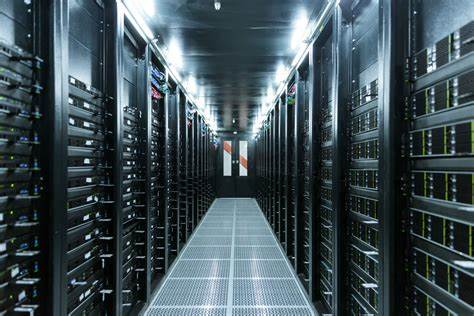
\includegraphics[scale=0.40]{images/3-1-1.jpg}
			\caption{大规模存储系统}
			\label{pic3-1-1}
		\end{center}
	\end{figure}
	\subsection{原理简述}
	大规模存储系统通常基于分布式存储架构构建。其核心原理是将数据分散存储在多个独立的存储节点上，这些节点通过高速网络进行连接。通过数据冗余技术，如副本冗余或纠删码冗余，保障数据的可靠性。当有数据写入请求时，系统会根据一定的算法（如一致性哈希算法）确定数据存储在哪些节点上，以实现数据的均匀分布和负载均衡。在数据读取时，系统能够快速定位数据所在节点并将其取回。同时，为了提高存储效率和管理便利性，会采用分层存储结构，将不同热度的数据分别存储在不同性能的存储介质上，例如将频繁访问的热数据存储在高速固态硬盘（SSD）中，而将访问频率较低的冷数据存储在大容量机械硬盘（HDD）中。
	
	\subsection{主要应用埸景}
	主要应用埸景\\
	1.	企业数据中心：\\
	企业利用大规模存储系统存储客户信息、交易记录、财务数据等各类业务数据，支持企业资源规划（ERP）、客户关系管理（CRM）等关键业务系统的运行，保障企业日常运营的连续性和数据安全性\\。
	2.	云存储服务：\\
	云服务提供商如亚马逊 AWS、微软 Azure、阿里云等基于大规模存储技术构建云存储平台，为广大用户和企业提供弹性可扩展的存储服务，用户可以按需租用存储资源，方便地存储和共享文件、备份数据等。\\
	3.	大数据分析：\\
	在大数据处理流程中，大规模存储系统作为数据的存储库，存储从各种数据源收集而来的海量数据，供数据挖掘、机器学习等大数据分析工具和算法进行处理，以提取有价值的信息和知识，例如电商企业分析用户购买行为数据来进行精准营销推荐。\\
	4.	媒体与娱乐行业：\\
	用于存储海量的影视、音乐、图片等媒体资源，满足在线视频播放平台、音乐流媒体服务、数字图书馆等的内容存储和分发需求，保障用户能够流畅地访问和欣赏各种媒体内容。\\
	
	
	\subsection{面对难题}
	面对难题\\
	1.性能瓶颈：\\数据量与应用需求增长致大规模存储系统读写遇阻，高并发时存储节点处理力与网络带宽成限制，使数据访问延迟，影响系统性能与用户体验。\\
	2.数据一致性：\\分布式存储下，数据于多节点分布，更新时同步机制若有差池易现数据不一致，危及数据准确可靠。\\
	3.扩展性挑战：\\虽设计可扩展，但实际添加存储节点或扩容量时，需对系统架构、数据分布策略与管理软件等调适优化，不然易现扩展后性能反降状况。\\
	4.数据安全与隐私：\\存大量敏感数据引黑客觊觎，有数据泄露、篡改风险，且数据共享使用时，需加密、访问控制等护隐私防滥用。\\
	

	\section{类脑计算机}
	(\ref{pic4-1-1})
	
	\begin{figure}[H]
	\begin{center}
		
\includegraphics[scale=0.40]{images/4-1-1.jpg}
		\caption{类脑计算机}
		\label{pic4-1-1}
	\end{center}
	\end{figure}
	\subsection{技术目的}
	技术目的\\
	1.突破传统计算架构瓶颈：\\传统冯诺依曼架构中存储器和处理器分离，限制了数据传输速度和处理效率，类脑计算机的设计旨在打破这种架构限制，探索新的计算模式，以满足现代社会对大数据处理、人工智能等领域日益增长的高性能计算需求\\
	2.模拟人脑高效能与低功耗特性：\\人脑在信息处理、学习、认知等方面展现出高效能和低功耗的优势，类脑计算机希望借鉴人脑的神经网络结构和工作原理，实现类似的高效信息处理能力，同时降低能耗，为可持续发展的智能计算提供解决方案\\
	3.推动人工智能发展：\\通过模拟人脑的神经元和突触等结构，构建更接近人类大脑的计算模型，有望实现更强大的人工智能，使计算机能够像人类一样进行学习、推理、决策等复杂的智能行为，从而在更多领域实现智能化应用
	
	\subsection{原理简述}
	模拟生物大脑神经网络结构与信息处理机制。一是神经元与突触模拟，以神经元为基本单元模拟信息收发整合及传递，借人工突触模拟生物突触特性构建大规模神经网络；二是脉冲神经网络，用脉冲信号传递信息，类似生物神经元工作方式，可处理非结构化数据，能效及时空处理能力佳；三是并行处理与分布式存储，仿人脑并行处理，众多神经元同时处理信息实现并行计算与快速响应，且采用分布式存储于神经元或存储单元中提升存储与访问效率。
	
	\subsection{主要应用埸景}
	主要应用埸景\\
	1.人工智能领域：\\为 AI 算法提供硬件支撑，加速模型训练与推理，提升语音、图像、自然语言处理等任务效能，助力其在智能语音助手等多领域应用拓展。\\
	2.大数据处理与分析：\\快速处理海量非结构化数据，挖掘信息知识，为企业商业智能等决策助力，应对大数据挑战。\\
	3.神经科学研究：\\作为工具，构建类脑模型与大脑数据对比验证，助神经科学家探索大脑奥秘，推动学科发展。\\
	4.机器人与智能控制：\\让机器人智能感知、决策与执行，增强自主性适应性，在多行业推动机器人技术应用。
	
	\subsection{面对难题}
	面对难题\\
	1.神经科学基础理论不足：\\人类对大脑认知尚缺，像意识、情感、创造力产生机制不明，致类脑计算机模型构建缺准确理论依据，难模拟大脑复杂功能，限制其技术发展。\\
	2.硬件技术限制：\\模拟大脑海量神经元与突触需先进硬件技术，当前芯片集成度、功耗、信号传输速度等方面有局限，制约类脑计算机规模与性能。\\
	3.软件与硬件协同困难：\\类脑计算需软硬件高度协同，可现实中硬件设计与软件开发较独立，缺沟通协同机制，系统优化、扩展及深度融合较难实现。\\
	4.能耗与散热问题：\\虽类脑计算机想模拟人脑低功耗特性，但因神经元网络规模大、计算复杂，仍能耗较高，且集成芯片器件多易生热，散热若不佳会影响稳定性与可靠性。\\
	5.系统可扩展性挑战：\\类脑计算机规模扩大时系统复杂性剧增，保证扩展中性能、数据、功能方面稳定完整是难题，不同规模、架构的兼容性与互操作性也需考量。
	
		
	\section{计算器通讯技术}
	\subsection{技术目的}
	1.实现信息高效共享与传递\ref{pic5-1-1}：\\打破地域限制，让不同地点的计算机之间能够快速、准确地传输各种数据信息，如文本、图像、音频、视频等，从而实现信息的广泛共享和高效流动，提高人们获取和处理信息的效率。\\
	\begin{figure}[H]
		\begin{center}
			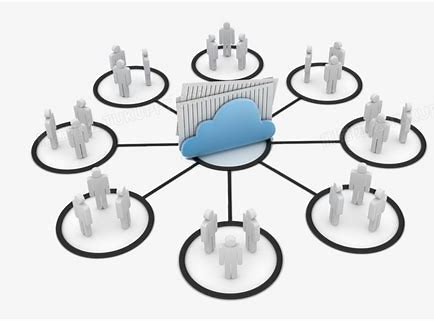
\includegraphics[scale=0.40]{images/5-1-1.jpg}
			\caption{信息高效共享与传递}
			\label{pic5-1-1}
		\end{center}
	\end{figure}
	2.支持分布式计算\ref{pic5-1-2}与协同工作：\\使多台计算机能够协同工作，共同完成复杂的计算任务或项目。通过计算机通讯技术，可以将大型任务分解到不同的计算机上进行处理，然后再将结果汇总，提高计算能力和工作效率，促进团队协作和资源共享。\\
	\begin{figure}[H]
		\begin{center}
			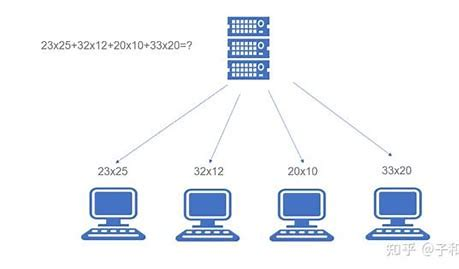
\includegraphics[scale=0.40]{images/5-1-2.jpg}
			\caption{分布式计算}
			\label{pic5-1-2}
		\end{center}
	\end{figure}
	3.构建全球互联网络：\\将世界各地的计算机网络连接在一起，形成一个庞大的全球性网络，即互联网。这使得人们能够跨越国界和地域进行即时通讯、信息交流和资源共享，推动了全球化的发展，促进了不同地区、不同文化之间的交流与合作。\\
	\begin{figure}[H]
		\begin{center}
			
\includegraphics[scale=0.40]{images/5-1-3.jpg}
			\caption{全球互联网络}
			\label{pic5-1-3}
		\end{center}
	\end{figure}
	4.满足多样化的应用需求：\\为各种应用场景提供通信基础，如企业的远程办公、在线教育、电子商务、远程医疗、智能交通等领域。这些应用都依赖于计算机通讯技术来实现数据的传输和交互，从而为人们的生活和工作带来更多的便利和创新。
	\begin{figure}[H]
		\begin{center}
			
\includegraphics[scale=0.40]{images/5-1-4.jpg}
			\caption{分布式计算}
			\label{pic5-1-4}
		\end{center}
	\end{figure}
	
	\subsection{原理简述}
	原理简述\\
	1.信号转换与传输：\\计算机内为数字信号，通信时要转为适合介质传输的信号（如电、光信号），发送端用调制技术转模拟信号传，接收端解调还原为数字信号供处理。\\
	2.数据编码与解码：\\数据先转二进制代码传输，接收方再解码还原。常见编码方式有 ASCII 码、Unicode 码等，用于将各类信息转为二进制数据。\\
	3.分组交换与路由选择：\\数据传输时分成数据包，含源地址、目的地址、数据等，经路由器依目的地址和网络拓扑选最佳路径转发，实现分组交换与路由传输。\\
	4.协议与分层架构：\\计算机通讯依分层协议，如 TCP/IP 协议族含多层面，各层负责不同功能，协同保障数据可靠、正确传输。
	
	
	\subsection{主要应用埸景}
	主要应用埸景\\
	1.互联网应用：\\是互联网运行基础，支持网页浏览、电子邮件等多种服务，便于全球信息交流互动。\\
	2.企业信息化：\\企业借计算机通讯技术构建内网，实现办公自动化、资源共享等，提升运营效率与管理水平，降成本、增竞争力。\\
	3.云计算与大数据：\\为其提供数据传输和存储支持，能将大量数据传至云端处理，用户可随时网络访问使用，实现数据集中管理高效利用。\\
	4.物联网：\\让物联网设备相互连接通信，实现智能化协同工作，像智能家居远程控制、智能交通提升效率与安全。\\
	5.远程监控与控制：\\在多领域借助该技术实现远程设备、系统实时监控与操作，提高生产效率与管理便捷性。
	
	
	\subsection{面对难题}
	面对难题\\
	1.网络安全威胁：\\计算机通讯技术广泛应用，网络安全问题凸显，像黑客攻击等，保障安全成重要挑战，需加强加密、身份认证等防护技术研发应用。\\
	2.网络拥塞与性能优化：\\数据流量增加致网络拥塞，出现传输延迟、丢包率升等问题，需从网络拓扑、带宽分配等多方面优化，提升承载和传输效率。\\
	3.兼容性与互操作性：\\不同计算机系统、设备、协议存在兼容及互操作问题，影响互联互通，要制定标准规范，推动厂商合作兼容，保障无缝对接协同。\\
	4.移动性与无线通信挑战：\\移动设备普及使无线通信占比增大，但面临信号干扰、覆盖及速率不稳定等难题，还需满足低功耗等要求，提高其质量性能是关键。\\
	5.新兴技术融合的复杂性：\\计算机通讯与人工智能等新兴技术融合，虽带来创新应用，却增加复杂性和实施难度，需跨领域人才团队协同研发推动落地应用。
	
	
	\section{通用人工智能的技术进展和典型应用}
	先前經已介紹了人工智能的定義和發展史，故在此不作展開，下面將以近代人工智能的技術進展和應用及更再說明面下挑戰以說明
	\subsection{技术進展}
	技术進展\\
	1.深度学习的深化：\\深度学习算法不断优化，模型规模和性能持续提升，如 OpenAI 的 GPT 系列，参数量和训练数据规模不断增大，使其语言理解和生成能力大幅提高，能够更好地处理复杂的自然语言任务。\\
	2.强化学习的应用拓展：\\在机器人控制、游戏等领域，强化学习让智能体能够通过与环境的交互不断学习和优化行为策略，取得了显著成果，如 AlphaGo Zero 通过自我对弈掌握围棋策略。\\
	3.知识图谱与推理技术：\\知识图谱构建不断完善，将海量的知识进行结构化表示和关联，结合神经符号系统等推理技术，使人工智能能够更好地进行跨领域知识融合与推理，理解和解决复杂问题。\\
	4.多模态融合技术：\\实现图像、语音、文本等多种模态信息的融合处理，让人工智能能够更全面地感知和理解世界，例如通过图像和文本的联合理解生成更准确的描述和回答。\\
	5.人工智能伦理与安全技术的探索：\\随着通用人工智能的发展，伦理和安全问题日益受到关注，研究人员正在探索可解释性 AI、道德约束算法等技术，以确保 AI 的决策透明、公平，防止其被恶意利用。
	\subsection{典型应用}
	典型应用\\
	1.医疗领域：\\
	辅助诊断方面，通用人工智能可通过学习分析大量医疗影像、病历等数据，助力医生开展疾病诊断与鉴别诊断，像在肺癌、乳腺癌等疾病的影像诊断中能提高准确性与效率。
	在个性化治疗方案制定上，依据患者基因数据、病史等个体特征，为其定制包含药物选择、治疗计划制定等在内的个性化方案，以此提高治疗效果并减少并发症。
	医疗机器人可用于辅助手术、康复训练等，例如达芬奇外科机器人能执行复杂微创手术，提升手术精准度、成功率，同时降低手术风险。\\
	2.教育领域：\\
	智能导师系统会依照学生的学习进度、兴趣爱好以及学习风格等，为其规划个性化学习路径、推荐学习内容，实时答疑并给予针对性辅导和反馈，以增强学习效果。
	语言学习辅助借助模拟真实语言交流场景，运用语音识别和自然语言生成技术等，助力学生提升语言听说读写能力，比如用于口语练习和写作指导。\\
	3.交通领域：\\
	自动驾驶技术依靠计算机视觉、传感器融合、深度学习等，让车辆自主感知周边环境，进行决策并控制行驶，像 Waymo 的自动驾驶汽车已在多城市测试运营，可提高交通安全性与出行效率。
	智能交通管理利用人工智能算法实时监测和预测交通流量，优化交通信号控制，缓解交通拥堵，提升城市交通运行效率。\\
	4.金融领域：\\
	风险评估与投资决策环节，通用人工智能分析海量金融市场数据、用户行为数据等，预测市场趋势与风险，为投资者和金融机构提供决策支撑，助力制定合理投资策略与风险管理方案。
	欺诈检测运用机器学习和数据挖掘技术，实时监控金融交易异常行为，及时察觉并防范欺诈活动，保障金融交易安全。\\
	5.制造业领域：\\
	智能生产与质量控制能够实现生产线自动化、智能化调度，优化生产流程，提高生产效率与产品质量，例如借助图像识别技术检测产品外观缺陷并及时处理。
	预测性维护基于传感器收集的设备运行数据来预估设备故障，提前安排维护计划，减少设备停机时间和维修成本，增强设备可靠性与可用性。
	
	\subsection{面对难题}
	面对难题\\
	1.数据相关\\
	数据获取成本与质量：\\高质量的标注数据对于许多人工智能算法尤其是深度学习至关重要，但获取大量标注数据往往需要耗费大量人力、物力和时间成本。例如在医疗影像标注中，需要专业医生来进行标注，过程极为繁琐。并且，数据质量参差不齐，存在错误标注、数据缺失、数据偏差等问题，这会影响模型训练效果，导致模型泛化能力不佳。\\
	数据隐私与安全：\\随着数据量和数据价值的不断提升，数据隐私和安全问题愈发凸显。一方面，在收集个人相关数据（如医疗数据、金融数据等）用于训练模型时，容易出现数据泄露风险，侵犯用户隐私。另一方面，恶意攻击者可能会篡改训练数据，使模型学习到错误的模式，进而影响模型输出的准确性和可靠性。\\
	\\2.模型性能相关\\
	泛化能力局限：\\当前人工智能模型在训练数据集中表现良好，但面对新的、未见过的数据或环境时，泛化能力常常不足。比如一个在特定场景图像识别准确率很高的模型，换到稍有差异的新场景中，识别准确率就会大幅下降，难以灵活应对多样化的现实情况。\\
	可解释性难题：\\许多先进的人工智能模型（如深度神经网络）如同“黑箱”，很难理解其内部决策过程和依据。在一些对可靠性要求极高的领域，像医疗诊断、金融风控等，无法解释模型为何做出某个决策，会导致用户（医生、投资者等）难以信任和采用该模型的结果。\\
	\\3.计算资源相关\\
	硬件算力需求：\\复杂的人工智能模型训练和推理需要强大的计算能力支持，例如训练超大规模的深度学习模型可能需要大量的图形处理单元（GPU）集群，耗费高昂的硬件成本以及大量的电力资源，这对很多研究机构和企业来说是个不小的负担，限制了模型研发和应用的规模与速度。\\
	能源消耗问题：\\人工智能计算过程耗能巨大，尤其随着模型复杂度不断增加，能源消耗呈上升趋势。从可持续发展角度看，如何降低其能源消耗，使其更环保、更高效地运行，是亟待解决的问题。
	\\4.算法与架构相关\\
	算法创新瓶颈：\\目前常用的人工智能算法在某些方面逐渐遇到发展瓶颈，如传统机器学习算法在处理高维、复杂非线性数据时的局限性，深度学习算法在提升效率、减少参数量同时保证性能等方面面临挑战，急需新的、更具突破性的算法出现。\\
	架构适应性不足：\\现有模型架构大多是针对特定任务或领域设计的，缺乏通用性和灵活性，难以适应快速变化、多任务融合的现实应用场景，很难做到像人类大脑一样自如地切换并处理不同类型的任务。
	\\5.伦理与法律相关\\
	算法偏见与公平性：\\由于训练数据本身存在的偏差或者模型设计等原因，人工智能系统可能会产生算法偏见，对不同性别、种族、地域等群体做出不公平的决策，比如在招聘推荐、信贷审批等场景中出现不合理的差异对待，违背了公平公正的社会伦理原则。\\
	责任界定困难：\\当人工智能系统做出错误决策或引发不良后果时，很难清晰界定是开发者、使用者还是系统本身的责任，例如自动驾驶汽车发生事故时，责任归属复杂，这需要完善的法律和伦理框架来明确各方的责任范围。
	

	\section{工程伦理}
	
	\subsection{技术目的}
	技术目的\\
	1.保障公众安全与福祉：\\工程伦理的设计旨在确保工程活动不会对公众的生命、健康和财产安全构成威胁，同时要积极促进社会福祉。例如，在建筑工程中，通过制定伦理准则来规范设计和施工过程，保证建筑物的质量和安全性。\\
	2.维护环境可持续性：\\引导工程师在进行工程活动时考虑对生态环境的影响，促使工程项目采用环保材料、减少污染排放等措施，实现工程与自然的和谐共生。如在水利工程建设中，考虑对河流生态系统的保护。\\
	3.促进公平与公正：\\保证工程决策和实施过程中的公平性，包括利益分配公平、机会公平等。在资源分配型工程（如城市供水工程）中，要确保不同地区、不同群体都能公平地获取资源。\\
	4.规范工程行为和职业操守：\\为工程师提供明确的行为准则，使其在面对复杂的工程问题和利益冲突时，能够做出符合道德的选择，维护工程行业的声誉和公信力。\\
	
	\subsection{原理简述}
	原理简述\\
	1.以伦理原则为基础的价值判断：\\工程伦理基于一系列基本伦理原则，如尊重人的尊严和权利、不伤害原则、公正原则、责任原则等。在工程活动中，对各种方案和行为进行评估，判断其是否符合这些伦理原则。例如，判断一个化工项目是否会对周边居民的健康造成伤害，是否公平地对待了所有利益相关者。\\
	2.利益相关者分析与平衡：\\识别工程活动中的所有利益相关者，包括投资者、工程师、工人、用户、社区居民、政府监管部门等。分析每个利益相关者的利益诉求、权利和责任，在工程决策过程中权衡各方利益，避免牺牲某一方的利益来满足另一方的利益。例如，在城市更新项目中，要平衡开发商的经济利益、居民的居住权益和城市的整体规划利益。
	\subsection{主要应用埸景}
	1.工程项目决策：\\在工程项目的前期规划阶段，运用工程伦理进行决策评估。例如，通过伦理审查来判断一个新的交通基础设施项目是否符合社会公平原则，是否会对环境造成不可接受的破坏，从而为项目的可行性提供伦理依据。\\
	2.工程设计优化：\\在工程设计中融入伦理考量，使设计方案更具人性化和可持续性。例如，在产品设计中考虑产品的可回收性，以减少对环境的影响；在建筑设计中考虑无障碍设施，以方便残障人士使用。\\
	3.工程教育与培训：\\在工程专业的教育体系中，将工程伦理作为重要的教学内容。通过案例教学、课堂讨论等方式，培养未来工程师的伦理意识和道德判断能力。例如，在工科院校的课程中设置工程伦理案例分析课程，让学生学会如何在工程实践中运用伦理原则。
	
	\subsection{面对难题}
	面对难题\\
	1.伦理标准的模糊性和多样性：\\不同文化、行业、组织和个人对工程伦理标准的理解和要求可能存在差异，导致在具体工程实践中难以确定统一的伦理标准。例如，对于转基因工程，不同国家和文化群体可能有不同的伦理态度。\\
	2.利益冲突的复杂性：\\工程活动涉及多个利益相关者，他们的利益诉求可能相互冲突，而且这些冲突往往很难协调。例如，在一个大型工业项目中，企业的经济效益、当地居民的生活质量和环境保护要求之间可能存在尖锐的矛盾。\\
	3.责任界定的困难性：\\在工程事故或问题发生后，很难准确界定工程师、企业管理者、政府监管部门等各方的伦理责任。例如，在建筑工程质量事故中，可能涉及设计缺陷、施工质量问题、材料质量问题和监管不力等多种因素，很难确定每个因素应承担的责任比例。\\
	4.技术发展带来的新伦理挑战：\\随着新兴技术（如人工智能、基因编辑、纳米技术等）的快速发展，不断出现新的伦理问题，而现有的工程伦理理论和方法可能无法及时应对这些问题。例如，人工智能算法中的偏见可能导致不公平的决策，如何从工程伦理角度解决这个问题是一个新的挑战。
	
	\section{總結心得}
	在完成计算机相关课程学习后，我对该领域有了深入且多面的认识。\\
	计算机与人工智能领域在科技的演进中经历了深刻的变革与发展。从早期传统计算机架构的构建，逐步形成了相对成熟的计算体系，在数据处理、信息存储等方面发挥了巨大作用。然而，随着时代的推进，数据量呈爆炸式增长，应用场景愈发复杂多样，传统架构在运算速度、存储容量以及能耗等方面逐渐暴露出瓶颈。这一困境促使科研人员积极探索新的计算模式，量子计算、神经形态计算等概念应运而生，它们在传统计算理论的基础上大胆创新，试图打破现有局限。\\
	大规模存储系统的分布式架构为应对海量数据存储提供了有效方案，其分散存储的方式增强了系统可靠性与扩展性，但数据一致性维护、节点与网络异常处理等挑战始终存在，要求开发者精心雕琢架构细节并制定周全策略。类脑计算机融合多学科智慧，致力于模拟大脑运作，可当前大脑认知的模糊性、硬件技术的滞后性以及软硬件协同的复杂性，使其发展之路布满荆棘，亟待跨学科的深度协作与技术攻坚。计算机通讯技术虽让世界紧密相连，却饱受网络拥塞、兼容性困扰以及移动无线通信固有难题的折磨，持续创新优化以构建稳定高效网络迫在眉睫。通用人工智能在多领域广泛渗透的同时，数据隐私泄露、算法可解释性缺失、社会就业结构冲击以及伦理道德争议等问题纷至沓来，呼唤着完善的监管体系与多因素综合权衡的发展思路。工程伦理在计算机与人工智能领域本应扮演重要角色，却因实践中伦理标准的模糊性而面临挑战，从业者强化伦理意识并融入决策过程对行业可持续发展至关重要。\\
	就我而言，我認為人工智能的道德伦理问题是存在的，令人忧心忡忡。在其自主性与决策能力日益强大的今天，缺乏明确道德准则的约束，其决策过程充满了不确定性与潜在风险。想象一下，在医疗资源紧张的情况下，人工智能系统可能因数据偏差而错误地分配资源，导致患者无法得到及时救治；在交通场景中，自动驾驶汽车面临两难抉择时，其决策依据若不遵循人类公认的道德原则，可能会造成不可挽回的伤亡事故。这一系列可能出现的情况都警示着我们，必须尽快确立一套严谨且普适的人工智能道德规范体系，从算法设计、数据采集到实际应用的各个环节，都要将伦理考量贯穿其中。同时，计算机硬件作为人工智能的物质基础，其发展水平的限制也不容忽视。当下硬件在运算速度、存储容量等方面的不足，使得人工智能在处理复杂数据和运行大型模型时捉襟见肘，严重制约了其智能水平的进一步提升。这让我深刻认识到，在追求人工智能软件创新的热潮中，不能忽视硬件技术的研发与突破。只有在确保软硬件协同共进的基础上，将人工智能的发展严格框定在道德伦理的轨道内，才能使其真正成为推动人类社会进步的强大动力，而非引发社会危机与人类价值冲突的根源。
	
%	\section{參考文獻}
%	以下為參考文獻：\\
 %   1.卢萍，李开，王多强，甘早斌.C语言程序设计典型题解与实验指导,北京:清华大学出版社,2019\\
  %  2.卢萍，李开，王多强，甘早斌.C语言程序设计,北京:清华大学出版社,2019
	
%	\section{网页整体框架}
	
%	实验室近期发表的一些论文\cite{Li2022AAAI, Chen2021MMA, Chen2022IMC, Ren2021JVCI, Ren2022MTAP}，欢迎同学们加入我们课题组做一些人工智能、计算机视觉、深度学习方面的一些有趣的课题！如果编译时候忘记关掉pdf文档造成编译出错，甚至不能再次编译，可以试试删除.bbl文件。图\ref{fig1-1}只是网页整体框架举例，它是用visio画的，然后再在visio里通过文件-打印，如图\ref{fig1-2}所示打印成pdf文件，然后再用pdf阅览器的工具，如图\ref{fig1-3}所示，做适当的裁剪。画图说明网页的整体框架，进行简要的文字描述等。画图说明网页的整体框架，进行简要的文字描述等。画图说明网页的整体框架，进行简要的文字描述等。画图说明网页的整体框架，进行简要的文字描述等。画图说明网页的整体框架，进行简要的文字描述等。画图说明网页的整体框架，进行简要的文字描述等。画图说明网页的整体框架，进行简要的文字描述等。
	
%	请注意，当正文中出现1) 2) 3)罗列时，请必须用enumerate环境，具体如下！
	
%	\begin{enumerate}
%		\renewcommand{\labelenumi}{\theenumi)}
%		\item C++
%		\item Java
%		\item HTML
%	\end{enumerate}
	
%	文档插图请放在images文件夹里。送给每人两千万：在html中千万不要搞错了路径，千万不要用绝对路径。画图说明网页的整体框架，进行简要的文字描述等。画图说明网页的整体框架，进行简要的文字描述等。画图说明网页的整体框架，进行简要的文字描述等。画图说明网页的整体框架，进行简要的文字描述等。画图说明网页的整体框架，进行简要的文字描述等。画图说明网页的整体框架，进行简要的文字描述等。画图说明网页的整体框架，进行简要的文字描述等。
	
%	\subsection{怎么加参考文献}
	
%	大力出奇迹！！！参考文献无法显示怎么办？陈老师正在想办法解决\cite{STR2021Neurocom, AVS2021Neurocom}！我是参考文献。我是第二小节\cite{Mehrabian1974An}。我是第二小节\cite{Rezaei2014CVPR}。我是第二小节\cite{Ramnath2008IJCV}。
	
%	先在文件夹里的bib文件里添加新的参考文献，给每篇参考文献取一个索引的名字，然后再引用比如\cite{STR2021Neurocom}\cite{AVS2021Neurocom, Rezaei2014CVPR}。请注意书籍、期刊论文、专利等bib条目的格式是不一样的。画图说明网页的整体框架，进行简要的文字描述等。画图说明网页的整体框架，进行简要的文字描述等。画图说明网页的整体框架，进行简要的文字描述等。画图说明网页的整体框架，进行简要的文字描述等。画图说明网页的整体框架，进行简要的文字描述等。画图说明网页的整体框架，进行简要的文字描述等。画图说明网页的整体框架，进行简要的文字描述等。
	
%	画图说明网页的整体框架，进行简要的文字描述等。画图说明网页的整体框架，进行简要的文字描述等。画图说明网页的整体框架，进行简要的文字描述等。画图说明网页的整体框架，进行简要的文字描述等。画图说明网页的整体框架，进行简要的文字描述等。画图说明网页的整体框架，进行简要的文字描述等。画图说明网页的整体框架，进行简要的文字描述等。
	
%	画图说明网页的整体框架，进行简要的文字描述等。画图说明网页的整体框架，进行简要的文字描述等。画图说明网页的整体框架，进行简要的文字描述等。画图说明网页的整体框架，进行简要的文字描述等。画图说明网页的整体框架，进行简要的文字描述等。画图说明网页的整体框架，进行简要的文字描述等。画图说明网页的整体框架，进行简要的文字描述等。
	
%	\begin{figure}[htb] % here top bottom
%		\begin{center}
%			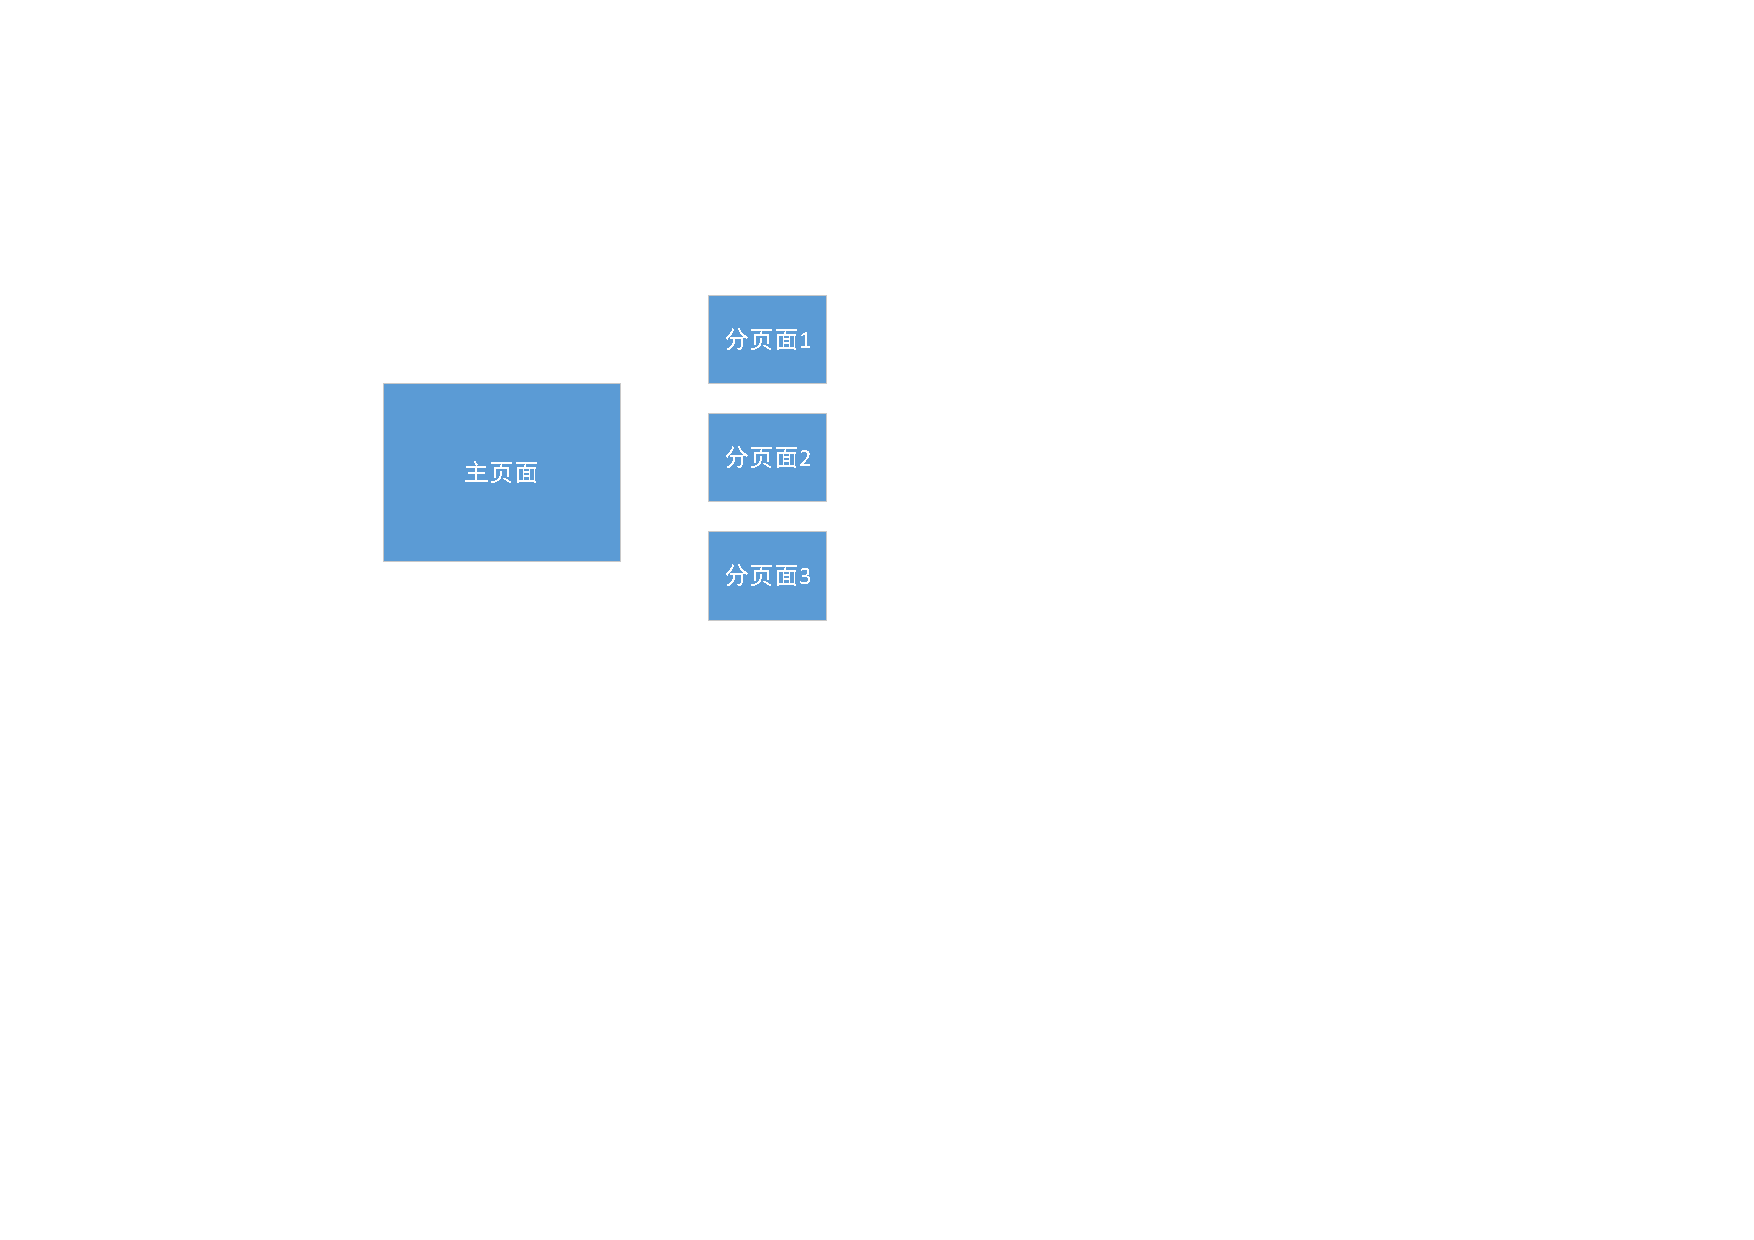
\includegraphics[scale=0.80]{images/1-1.pdf}
%			\caption{网页整体框架举例}
%			\label{fig1-1}
%		\end{center}
%	\end{figure}
	
%	画图说明网页的整体框架，进行简要的文字描述等。画图说明网页的整体框架，进行简要的文字描述等。画图说明网页的整体框架，进行简要的文字描述等。画图说明网页的整体框架，进行简要的文字描述等。画图说明网页的整体框架，进行简要的文字描述等。画图说明网页的整体框架，进行简要的文字描述等。画图说明网页的整体框架，进行简要的文字描述等。
	
%	\begin{figure}[htb]
%		\begin{center}
%			
\includegraphics[scale=0.60]{images/1-2.png}
%			\caption{在visio里通过文件-打印，把visio图打印成pdf文件}
%			\label{fig1-2}
%		\end{center}
%	\end{figure}
	
%	画图说明网页的整体框架，进行简要的文字描述等。画图说明网页的整体框架，进行简要的文字描述等。画图说明网页的整体框架，进行简要的文字描述等。画图说明网页的整体框架，进行简要的文字描述等。画图说明网页的整体框架，进行简要的文字描述等。画图说明网页的整体框架，进行简要的文字描述等。画图说明网页的整体框架，进行简要的文字描述等。
	
%	\begin{figure}[htb]
%		\begin{center}
%			
\includegraphics[scale=0.50]{images/1-3.png}
%%			\caption{用pdf阅览器的工具，对打印得到pdf图做适当的裁剪}
%			\label{fig1-3}
%		\end{center}
%	\end{figure}
	
%	画图说明网页的整体框架，进行简要的文字描述等。画图说明网页的整体框架，进行简要的文字描述等。画图说明网页的整体框架，进行简要的文字描述等。画图说明网页的整体框架，进行简要的文字描述等。画图说明网页的整体框架，进行简要的文字描述等。画图说明网页的整体框架，进行简要的文字描述等。画图说明网页的整体框架，进行简要的文字描述等。
	
%	\newpage
	
%	\section{主页设计}
	
%	描述主页的结构，给出主页截图，描述主要设计思路等，请见图\ref{fig2-1}。描述主页的结构，给出主页截图，描述主要设计思路等。描述主页的结构，给出主页截图，描述主要设计思路等。描述主页的结构，给出主页截图，描述主要设计思路等。描述主页的结构，给出主页截图，描述主要设计思路等。描述主页的结构，给出主页截图，描述主要设计思路等。描述主页的结构，给出主页截图，描述主要设计思路等。
	
%	\begin{figure}[htb]
%		\begin{center}
%			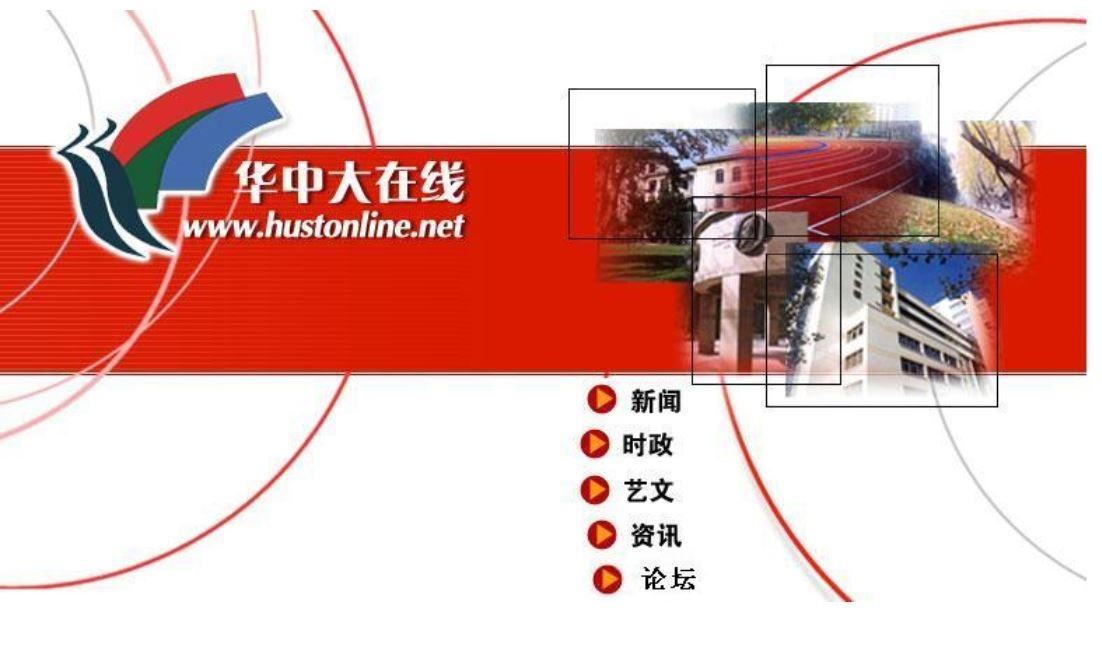
\includegraphics[scale=0.40]{images/2-1.jpg}
%			\caption{主页举例}
%			\label{fig2-1}
%		\end{center}
%	\end{figure}
	
%	描述主页的结构，给出主页截图，描述主要设计思路等。描述主页的结构，给出主页截图，描述主要设计思路等。描述主页的结构，给出主页截图，描述主要设计思路等。描述主页的结构，给出主页截图，描述主要设计思路等。描述主页的结构，给出主页截图，描述主要设计思路等。描述主页的结构，给出主页截图，描述主要设计思路等。描述主页的结构，给出主页截图，描述主要设计思路等。
	
%	描述主页的结构，给出主页截图，描述主要设计思路等。描述主页的结构，给出主页截图，描述主要设计思路等。描述主页的结构，给出主页截图，描述主要设计思路等。描述主页的结构，给出主页截图，描述主要设计思路等。描述主页的结构，给出主页截图，描述主要设计思路等。描述主页的结构，给出主页截图，描述主要设计思路等。描述主页的结构，给出主页截图，描述主要设计思路等。
	
%	描述主页的结构，给出主页截图，描述主要设计思路等。描述主页的结构，给出主页截图，描述主要设计思路等。描述主页的结构，给出主页截图，描述主要设计思路等。描述主页的结构，给出主页截图，描述主要设计思路等。描述主页的结构，给出主页截图，描述主要设计思路等。描述主页的结构，给出主页截图，描述主要设计思路等。描述主页的结构，给出主页截图，描述主要设计思路等。
	
%	描述主页的结构，给出主页截图，描述主要设计思路等。描述主页的结构，给出主页截图，描述主要设计思路等。描述主页的结构，给出主页截图，描述主要设计思路等。描述主页的结构，给出主页截图，描述主要设计思路等。描述主页的结构，给出主页截图，描述主要设计思路等。描述主页的结构，给出主页截图，描述主要设计思路等。描述主页的结构，给出主页截图。
	
%	\newpage
	
%	\section{分页面设计}
	
%	给出分页面截图，描述主要设计思路等。给出分页面截图，描述主要设计思路等。给出分页面截图，描述主要设计思路等。给出分页面截图，描述主要设计思路等。
	
%	\subsection{页面1 (每个页面以主要内容起标题名称即可）}
	
%	给出分页面截图，描述主要设计思路等。给出分页面截图，描述主要设计思路等。给出分页面截图，描述主要设计思路等。给出分页面截图，描述主要设计思路等。给出分页面截图，描述主要设计思路等。给出分页面截图，描述主要设计思路等。给出分页面截图，描述主要设计思路等。给出分页面截图，描述主要设计思路等。给出分页面截图，描述主要设计思路等。给出分页面截图，描述主要设计思路等。给出分页面截图，描述主要设计思路等。给出分页面截图，描述主要设计思路等。给出分页面截图，描述主要设计思路等。
	
%	如果实验报告中要用到算法伪代码，请参考算法\ref{alg:1}，也可以参考算法\ref{alg:2}。如果实验报告中要用到算法伪代码，请参考算法\ref{alg:1}，也可以参考算法\ref{alg:2}。如果实验报告中要用到算法伪代码，请参考算法\ref{alg:1}，也可以参考算法\ref{alg:2}。如果实验报告中要用到算法伪代码，请参考算法\ref{alg:1}，也可以参考算法\ref{alg:2}。
	
%	\begin{shaded*}\begin{alg}{一个复杂算法}
%			\label{alg:1}
%			\begin{algorithmic}
%				\Input Two numbers $a$ and $b$
%				\Output The sum of $a$ and $b$
%				\Procedure{A-Plus-B}{$a, b$}
%				\If $a = 0$
%				\State \Return $b$
%				\EndIf
%				\State $res \gets 0$
%				\While{$b \neq 0$}
%				\State Increase $res$ by $1$
%				\State $b \gets b - 1$
%				\EndWhile
%				\State \Return $res$
%				\EndProcedure
%			\end{algorithmic}
%	\end{alg}\end{shaded*}
%	
%	\subsection{页面2 (每个页面以主要内容起标题名称即可）}
	
%	给出分页面截图，描述主要设计思路等。给出分页面截图，描述主要设计思路等。给出分页面截图，描述主要设计思路等。给出分页面截图，描述主要设计思路等。给出分页面截图，描述主要设计思路等。给出分页面截图，描述主要设计思路等。给出分页面截图，描述主要设计思路等。给出分页面截图，描述主要设计思路等。给出分页面截图，描述主要设计思路等。给出分页面截图，描述主要设计思路等。给出分页面截图，描述主要设计思路等。
	
	
%	如果实验报告中要用到算法伪代码，请参考算法\ref{alg:1}，也可以参考算法\ref{alg:2}。如果实验报告中要用到算法伪代码，请参考算法\ref{alg:1}，也可以参考算法\ref{alg:2}。如果实验报告中要用到算法伪代码，请参考算法\ref{alg:1}，也可以参考算法\ref{alg:2}。如果实验报告中要用到算法伪代码，请参考算法\ref{alg:1}，华科计院不认同考算法\ref{alg:1}的格式，而认同具有三线表的算法\ref{alg:2}格式。
	
%	\begin{algorithm}[h] 
%		\caption{一个更复杂算法}
%		\begin{algorithmic}[1]
%			\State Initialization: $I_{xy}$, $z_{f}=Zeros(128, 128)$; 
%			\For{$0\leq n \textless N$}
%			\State $i=\lfloor x_n \rfloor+64$, $j=\lfloor y_n \rfloor + 64$
%			\If{$z_n<0$ and $|z_n|>|z_{f}(i,j)|$};
%			\State $z_{f}(i,j)=z_n$;
%			\EndIf
%			\State $I_{xy}(i,j)=z_{f}(i,j)$;
%			\EndFor 
%		\end{algorithmic}\label{alg:2}
%	\end{algorithm}
	
%	\subsection{页面3 (每个页面以主要内容起标题名称即可）}
	
%	给出分页面截图，描述主要设计思路等。给出分页面截图，描述主要设计思路等。给出分页面截图，描述主要设计思路等。给出分页面截图，描述主要设计思路等。给出分页面截图，描述主要设计思路等。给出分页面截图，描述主要设计思路等。给出分页面截图，描述主要设计思路等。给出分页面截图，描述主要设计思路等。给出分页面截图，描述主要设计思路等。给出分页面截图，描述主要设计思路等。给出分页面截图，描述主要设计思路等。
	
%	\subsection{页面4 (每个页面以主要内容起标题名称即可）}
	
%	给出分页面截图，描述主要设计思路等。给出分页面截图，描述主要设计思路等。给出分页面截图，描述主要设计思路等。给出分页面截图，描述主要设计思路等。给出分页面截图，描述主要设计思路等。给出分页面截图，描述主要设计思路等。给出分页面截图，描述主要设计思路等。给出分页面截图，描述主要设计思路等。给出分页面截图，描述主要设计思路等。给出分页面截图，描述主要设计思路等。给出分页面截图，描述主要设计思路等。
	
%	\newpage
	
%	\section{网页设计小结}
	
%	描述网页的设计和实现过程中遇到的问题及如何解决。描述网页的设计和实现过程中遇到的问题及如何解决。描述网页的设计和实现过程中遇到的问题及如何解决。描述网页的设计和实现过程中遇到的问题及如何解决。描述网页的设计和实现过程中遇到的问题及如何解决。描述网页的设计和实现过程中遇到的问题及如何解决。描述网页的设计和实现过程中遇到的问题及如何解决。描述网页的设计和实现过程中遇到的问题及如何解决。描述网页的设计和实现过程中遇到的问题及如何解决。
	
%	描述网页的设计和实现过程中遇到的问题及如何解决。描述网页的设计和实现过程中遇到的问题及如何解决。描述网页的设计和实现过程中遇到的问题及如何解决。描述网页的设计和实现过程中遇到的问题及如何解决。描述网页的设计和实现过程中遇到的问题及如何解决。描述网页的设计和实现过程中遇到的问题及如何解决。描述网页的设计和实现过程中遇到的问题及如何解决。描述网页的设计和实现过程中遇到的问题及如何解决。描述网页的设计和实现过程中遇到的问题及如何解决。
	
%	描述网页的设计和实现过程中遇到的问题及如何解决。描述网页的设计和实现过程中遇到的问题及如何解决。描述网页的设计和实现过程中遇到的问题及如何解决。描述网页的设计和实现过程中遇到的问题及如何解决。描述网页的设计和实现过程中遇到的问题及如何解决。描述网页的设计和实现过程中遇到的问题及如何解决。描述网页的设计和实现过程中遇到的问题及如何解决。描述网页的设计和实现过程中遇到的问题及如何解决。描述网页的设计和实现过程中遇到的问题及如何解决。
	
%	描述网页的设计和实现过程中遇到的问题及如何解决。描述网页的设计和实现过程中遇到的问题及如何解决。描述网页的设计和实现过程中遇到的问题及如何解决。描述网页的设计和实现过程中遇到的问题及如何解决。描述网页的设计和实现过程中遇到的问题及如何解决。描述网页的设计和实现过程中遇到的问题及如何解决。描述网页的设计和实现过程中遇到的问题及如何解决。描述网页的设计和实现过程中遇到的问题及如何解决。描述网页的设计和实现过程中遇到的问题及如何解决。
	
%	\newpage
	
%	\section{课程的收获和建议}
	
%	学习效率最好的方法，认真听讲，认真审题，认真模仿提供的例子。描述通过学习该专题，有何收获，有何建议，如某专题可适当减少讲授时间、某专题可适当增加讲授内容和时间等。描述通过学习该专题，有何收获，有何建议，如某专题可适当减少讲授时间、某专题可适当增加讲授内容和时间等。描述通过学习该专题，有何收获，有何建议，如某专题可适当减少讲授时间、某专题可适当增加讲授内容和时间等。描述通过学习该专题，有何收获，有何建议，如某专题可适当减少讲授时间、某专题可适当增加讲授内容和时间等。
	
%	\subsection{计算机基础知识}
	
%	描述通过学习计算机基础知识专题，有何收获，有何建议，如某专题可适当减少讲授时间、某专题可适当增加讲授内容和时间等。描述网页的设计和实现过程中遇到的问题及如何解决。描述网页的设计和实现过程中遇到的问题及如何解决。描述网页的设计和实现过程中遇到的问题及如何解决。描述网页的设计和实现过程中遇到的问题及如何解决。描述网页的设计和实现过程中遇到的问题及如何解决。描述网页的设计和实现过程中遇到的问题及如何解决。描述网页的设计和实现过程中遇到的问题及如何解决。描述网页的设计和实现过程中遇到的问题及如何解决。明年要讲一下什么是资源管理器，怎么新建文件夹与文件。怎么装正版的软件，特别是winrar。还要提前提醒大家不要装任何电脑管家。
	
%	\subsection{文档撰写工具LaTeX}
	
%	描述通过学习文档撰写工具LaTeX专题，有何收获，有何建议，如某专题可适当减少讲授时间、某专题可适当增加讲授内容和时间等。描述通过学习文档撰写工具LaTeX专题，有何收获，有何建议，如某专题可适当减少讲授时间、某专题可适当增加讲授内容和时间等。插入参考文献、表格、公式、图是LaTeX最基本的操作，考核题目不能再简单了。如何插入算法，需要大家对照提供的例子去模仿。还记得部分同学看到cmd窗口里``请按任意键继续''后手足无措的样子!
	
%	\subsection{编程工具Python}
	
%	Python讲都是基础知识，如果讲慢了，基础就讲不完了，讲快了部分同学们又跟不上，这个矛盾怎么解决？描述通过学习编程工具Python专题，有何收获，有何建议，如某专题可适当减少讲授时间、某专题可适当增加讲授内容和时间等。描述通过学习编程工具Python专题，有何收获，有何建议，如某专题可适当减少讲授时间、某专题可适当增加讲授内容和时间等。装环境、配解释器、矩阵运算、图像操作等是实际开发的利器，希望大家巩固掌握。Python语法就那么一点，基础入门并不难的。编程习惯很重要，胜过语法本身，部分同学还没有改掉用绝对路径的毛病！部分同学试图实现跨文件夹的import！出问题不可怕，可怕的是不按照规范来施行！
	
%	\subsection{图像设计软件Photoshop}
	
%	流程图一定要画的规范。Visio是画流程图的好帮手，记得在视图里勾上grid。描述通过学习Photoshop与Visio专题，有何收获，有何建议，如某专题可适当减少讲授时间、某专题可适当增加讲授内容和时间等。描述通过学习计算机基础知识专题，有何收获，有何建议，如某专题可适当减少讲授时间、某专题可适当增加讲授内容和时间等。同学们可以再这里贴上你骄傲的作品。课程内容相对较好，每个实践例子老师表演了2到3遍。部分进校时的小白同学通过课下温习，掌握的非常好。
	
%	\subsection{版本管理软件Git}
	
%	描述通过学习图像设计软件Git专题，有何收获，有何建议，如某专题可适当减少讲授时间、某专题可适当增加讲授内容和时间等。描述通过学习图像设计软件Photoshop专题，有何收获，有何建议，如某专题可适当减少讲授时间、某专题可适当增加讲授内容和时间等。先送给大家一千万：千万不能用中文注册github或者gitee的账号！add remote添加远程仓库是最容易出问题的地方，错误的种类千千万，操作正确的道路就一条。再送每人两千万：千万不要添加错了远程仓库的地址，不千万要搞混远程仓库地址中的用户名及其与之关联的字段。
	
%	\subsection{网页制作Dreamweaver}
	
%	描述通过学习网页制作Dreamweaver专题，有何收获，有何建议，如某专题可适当减少讲授时间、某专题可适当增加讲授内容和时间等。描述通过学习网页制作Dreamweaver专题，有何收获，有何建议，如某专题可适当减少讲授时间、某专题可适当增加讲授内容和时间等。还记得老师送的两千万吗？绝对路径千万不可取，资源路径千万要放在工作区！
	
	
%	\nocite{*} %% 作用是不对文献进行引用，但可以生成文献列表
	
%	\bibliographystyle{Experimental_Report}
%	\bibliography{Experimental_Report}
%	\setcounter{secnumdepth}{0}
%	\appendix
	
%	\section{附录A 功能模块一实现的主要源程序}
	
%	\noindent
%	/* Linear Table On Sequence Structure */\\
%	\#include <stdio.h>\\
%	\#include <malloc.h>\\
%	\#include <stdlib.h>\\
	
%	\noindent
%	/*---------page 10 on textbook ---------*/\\
%	\#define TRUE 1\\
%%	\#define FALSE 0\\
%	\#define OK 1\\
%	\#define ERROR 0\\
%	\#define INFEASTABLE -1\\
%	\#define OVERFLOW -2\\
%	\newpage
%	\section{附录B 功能模块二实现的主要源程序}
%	\newpage
%	\section{附录C 功能模块三实现的主要源程序}
%	\newpage
%	\section{附录D 功能模块四实现的主要源程序}
	
\end{document}